%! Author = rickr
%! Date = 11/17/2021
\newpage
\section{Traveling Salesman Problem To Ising Model}
	Recent interest in solving NP-complete and NP-hard problems via adiabatic quantum optimization has led to convenient transformations of Ising formulations. The idea is that if one problem has a quantum Hamiltonian $H_p$ whose ground state energy encodes the solution to a problem of interest, and another Hamiltonian $H_0$, whose ground state is "easy" to find and prepare, then we can prepare the system to be in the ground state of $H_0$ before adiabatically changing it in terms of $H_p$ for a time $T$ \cite{lucas2014ising}. So long as $T$ is large enough and $H_0$ and $H_p$ do not commute, the system should remain in the resulting ground state for all time. Therefore, measuring the ground state of the system at time $T$ will return a solution to the problem of interest. Though there has been debate on the practicality of such a method, there has been extensive effort in finding formulations of various NPC and NPH problems in terms of Ising models. Here we present one such transformation and show how it can be used to improve the computation time of a generic Branch-and-Bound technique. 
	\subsection{TSP to Hamiltonian Circuit}
		Consider an instance of the Traveling Salesman problem for the graph $G = (V,E)$ as shown in Figure \ref{fig:tsp}.
		Each edge $uv$ has a weight $W_{uv}$ associated with it. 
		\begin{figure}[h]
			\begin{center}
				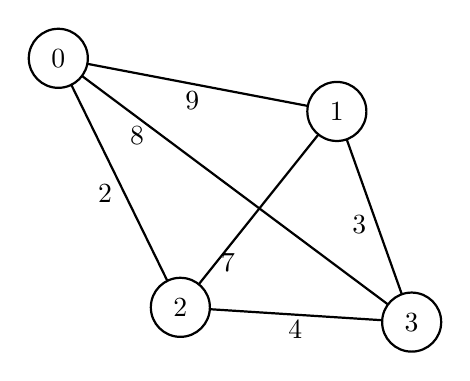
\begin{tikzpicture}[scale=0.125]
					\tikzstyle{every node}+=[inner sep=0pt]
					\draw  [thick](22,-14.2) circle (3);
					\draw  [][thick](22,-14.2) node {$0$};
					\draw  [thick](34.4,-39.5) circle (3);
					\draw  [][thick](34.4,-39.5) node {$2$};
					\draw  [thick](50.3,-19.6) circle (3);
					\draw  [][thick](50.3,-19.6) node {$1$};
					\draw  [thick](57.9,-41) circle (3);
					\draw  [][thick](57.9,-41) node {$3$};
					\draw  [][thick](23.32,-16.89) -- (33.08,-36.81);
					
					\draw [](27.5,-27.94) node [left] {$2$};
					\draw [][thick] (24.95,-14.76) -- (47.35,-19.04);
					
					\draw [](35.62,-17.49) node [below] {$9$};
					\draw [][thick] (51.3,-22.43) -- (56.9,-38.17);
					
					\draw [](53.34,-31.06) node [left] {$3$};
					\draw [][thick] (37.39,-39.69) -- (54.91,-40.81);
					
					\draw [](46.07,-40.81) node [below] {$4$};
					\draw [][thick] (24.4,-15.99) -- (55.5,-39.21);
					
					\draw [](30,-23) node [above] {$8$};
					\draw [][thick] (48.43,-21.94) -- (36.27,-37.16);
					
					\draw [](40, -35) node [left] {$7$};
				\end{tikzpicture}\caption{A graph G representing an instance of the Traveling Salesman Problem. Each node $V$ is connected via a weighted edge $E=W_{uv}$. }\label{fig:tsp}
			\end{center}
		\end{figure}\\
		The set of solutions to this graph can be seen in Table \ref{tab:eigenset} located in the appendix and the shortest Hamiltonian cycle that can be taken has a total distance of 18.
		One possible route is $2\rightarrow3\rightarrow1\rightarrow0$. 
		This route can be represented as a matrix as shown if Figure \ref{fig:matrix}, where $i$ and $p$ correspond to the city and order of traversal respectively. 
		\begin{figure}[h]
			\begin{center}
					\begin{tabular}{c|cccc}
					\backslashbox{i}{p}&0 &1 &2 &3 \\
					\hline
					0& 0&0&0&1\\
					
					1& 0&0&1&0\\
					
					2& 1&0&0&0\\
					
					3& 0&1&0&0\\
				\end{tabular}
			\end{center}\caption{Solution to TSP in Figure \ref{fig:tsp} represented in the form of a matrix. The column $i$ represents each node, and the row $p$ corresponds to the nodes position in the traversal. A decision variable value of 1 corresponds to the path being taken.}\label{fig:matrix}
		\end{figure}\\
		The solution matrix of Figure \ref{fig:matrix} can be unpacked into the form of a vector 
		\begin{equation}
			\vec{x} = \langle x_1, x_2, \dots, x_{N^2} \rangle
			\label{eq:vector}
		\end{equation}
		such that $x_j = x_{N \cdot i+p}$ where $N$ is the number of nodes in the graph. 
		For example, the value at $x_{2,1}$ in the matrix will map to $x_9$ in the vector. Therefore, the vector representation of the solution to TSP in Figure \ref{fig:tsp} is $\vec{x} = <0,0,0,1,0,0,1,0,1,0,0,0,0,1,0,0>$. 
		Applying the cost function to the eigenvector will result in an eigenvalue of $C(\vec{x}) = 18$.\\
		
		For nodes forming a traversal such that $x_{i,p}$ and $x_{i,p+1}$ are both equal to one but not connected in $G$, i.e., $(i,j)\notin E$, then an energy penalty should be imposed in the form $\sum_{i,j \notin E}\sum_p x_{i,p}x_{i,p+1}>0$ \cite{lucas2014ising}.
		However, since we are only considering fully connected graphs, this term may be omitted and the net cost of a tour can be calculated from the cost function of Equation \ref{eq:cost}.
		% Cost Function
		\begin{equation}
			C(X)=\sum_{i,j}w_{i,j} \sum_p x_{i,p}x_{j,p+1} 
			\label{eq:cost}
		\end{equation}
		Inspecting the features of Figure \ref{fig:matrix}, we find that every vertex can only appear once in a cycle and each position must be occupied by a node. 
		This amounts to the two constraints given in Equation \ref{eq:constraints}.
		% Constraints
		\begin{equation}
			\sum_p x_{i,p}=1 \quad \forall \: i \in cities \quad \text{and} \quad \sum_i x_{i,p}=1 \quad \forall \: p \in route
			\label{eq:constraints}
		\end{equation}
		By imposing these constraints to Equation \ref{eq:cost}, we find that the objective function to be minimized takes the form
		% Distance with constraints
		\begin{equation}
			C(X)=\sum_{i,j}w_{i,j} \sum_p x_{i,p}x_{j,p+1} + A\sum_p (1 - \sum_i x_{i,p})^2 + A\sum_i (1 - \sum_p x_{i,p})^2
			\label{eq:hamiltoniancircuit}
		\end{equation}
		where $A>W_{max}$ is a positive constant set to be much larger than maximum weight encountered during the traversal. Note that the constraints are squared so as to prevent the algorithm from diverging to negative infinity. \\
	
		To complete the preparation of TSP, we need to convert the cost function of Equation \ref{eq:cost} into a quantum Hamiltonian by changing variables from $x_i$ to the Pauli operator $\sigma_i^z$ (a $2x2$ matrix whose eigenvectors $|1,0\rangle$ and $|0,-1\rangle$ have eigenvalues (+1,-1)). 
		\begin{equation}
			x_i \rightarrow \frac{ 1-\sigma_{i,p}^z}{2} \qquad \Rightarrow \qquad C(X) \rightarrow C(\sigma_{i,p}^z) \equiv H_p
			\label{eq:transformation}
		\end{equation}
	
	\subsection{The Ising Model}
		In ideal \textit{paramagnetism} (magnetism where materials are weakly attracted by an external magnetic field) microscopic magnetic dipole moments respond only to an external field. 
		However, in the real world, neighboring atomic dipoles are influenced by each other. 
		When neighboring dipoles align parallel, even in the absence of an external field, we call the material a ferromagnet. 
		The Ising model is a mathematical model used to describe ferromagnetism in terms of statistical mechanics. The model consists of discrete variables that represent the magnetic dipole moments of atomic spins and can have a value of $\pm 1$. 
		The variables are used to describe preference for neighboring dipoles to align parallel or anti-parallel to each other \cite{schroeder2011thermal}.
		
		\begin{figure}[h]
			\begin{center}
				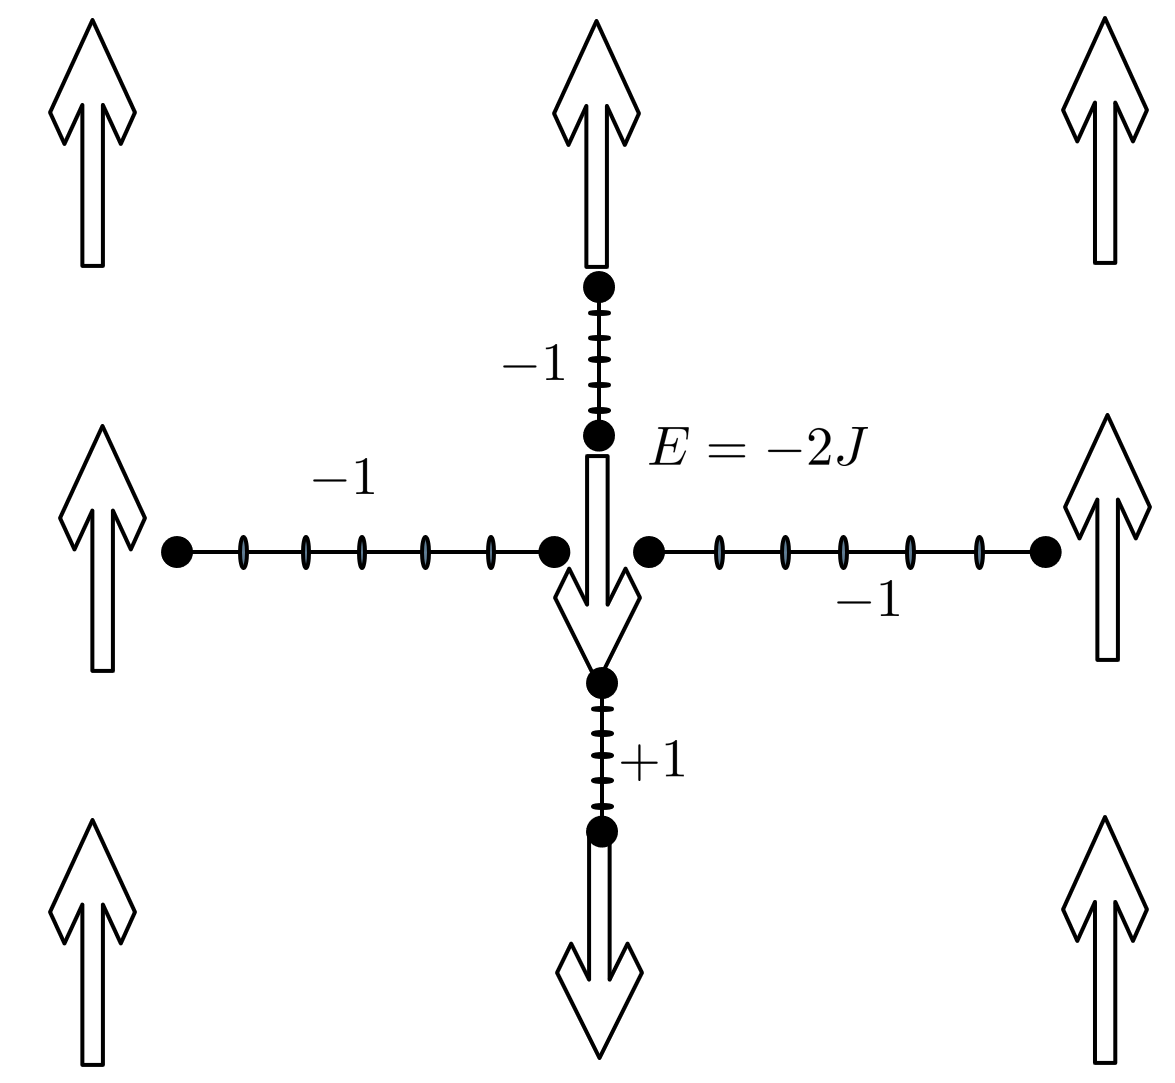
\includegraphics[width=4cm]{images/lattice}
			\end{center}
			\caption{Atomic spin states arranged into a 2-dimensional lattice structure under periodic boundary conditions. The energy of the particle at lattice site $k$ has a value $E = -2J$ and the total energy of the system is found by summing over the entire structure.}\label{fig:lattice}
		\end{figure}
	
		For example, consider a lattice of particles as shown in Figure \ref{fig:lattice}. 
		Each particle has an associated spin state that can take the orientations of spin-up $|+\rangle$ or spin-down $|-\rangle$ with values $\sigma_k = +1$ and $\sigma_k = -1$ respectively. The energy associated with the particle at lattice site $k$ is found to be 
		\begin{equation}
			 E_k= - J\sum_{<i,j>}\sigma_k^i\sigma_k^j \quad \cite{ising1925beitrag}
			\label{eq:latticeSiteEnergy}
		\end{equation}
		where $J$ is a coupling constant, $\sigma_k$ is a discrete variable, and $<i,j>$ means to sum over the nearest neighbors. Note that for parallel spins, $J>0$, for anti-parallel spins $J<0$, and for no interaction $J = 0$. 
		In the presence of a magnetic field $\vec{B}$, the kinetic and potential energy of the system can be represented by the Hamiltonian
		\begin{equation}
			H = \frac{g_s}{2}\mu_B B\sum_{i=1}^N \sigma_z^i - J\sum_{<i,j>}\sigma_z^i\sigma_z^j
			\label{eq:isingHamiltonian}
		\end{equation} 
		where the spin g-factor for an electron $g_s$ and the Bohr magneton $\mu_B$ are constants, and the discrete variable $\sigma_k$ has been replaced with the Pauli z-operator $\sigma_z$ as in Equation \ref{eq:transformation}. 
		There are many techniques for solving generalized Ising models including transfer matrix methods\cite{onsager1944crystal}, graphical/combinatorial methods\cite{feynman1972statistical}, and Monte Carlo simulations\cite{schroeder2011thermal}. 
		However, with the advent of quantum computation, the time independent Schrodinger equation is especially convenient.  
	\subsection{Time Independent Schrodinger Equation}
		In quantum mechanics, the Schrodinger equation is a partial differential equation that governs the dynamics of the wave function $\Psi(x,t)$ of a particle in a system. 
		In essence, it is an accounting of energy where the kinetic and potential energy are encapsulated in a single operator called a Hamiltonian, and the total energy of the system is set to be the time derivative acting on the wave function. 
		Since the Ising model focuses on the spin configuration of a particle and neglects the space and time components, we can utilize a time independent version of the Schrodinger equation and treat it as an eigenvalue problem as shown in Equation \ref{eq:tise}. 
		
		\begin{equation}
			H | \Psi \rangle = E | \Psi \rangle
			\label{eq:tise}
		\end{equation}
	
		As the Hamiltonian operator acts on the wave function, a scalar value is produced along with the same vector. 
		In terms of linear algebra, the wave function $| \Psi \rangle$ can be treated as an eigenvector with a corresponding eigenvalue $E$. 
		Note that each eigenvalue can correspond to a set of eigenvectors and that minimizing Equation \ref{eq:tise} is to solve for the ground state energy of the system. \\
		
		Relating this back to the Traveling Salesman problem, recall that in Equation \ref{eq:transformation} we transformed the cost function into the same form as the Ising Hamiltonial of Equation \ref{eq:isingHamiltonian}. We now need to map the solution vector of Equation \ref{eq:vector} into qubits to be fed into a quantum computer. 
		\begin{equation}
			\vec{x} = \langle x_1, x_2, \dots, x_{N^2} \rangle \rightarrow |\Psi\rangle = |x_1\rangle \otimes |x_2\rangle \dots \otimes  |x_{N^2}\rangle 
		\end{equation}
		Note that we do not require a transformation between the energy of the Schrodinger equation and the distance of the Hamiltonian Circuit because both quantities are scalars. This completes the transformation from the Traveling Salesman problem into the Ising model. The solution for the ground state energy of the Ising Hamiltonian corresponds directly to the minimum tour distance in TSP, however, in this form we are able to exploit the features of quantum mechanics and obtain a solution in far less time. 
